\section{背景：LLM 服务、KVCache、KVCache 缓存与多轮服务}
\label{sec:bg}

\begin{figure}[!t]
    \centering
    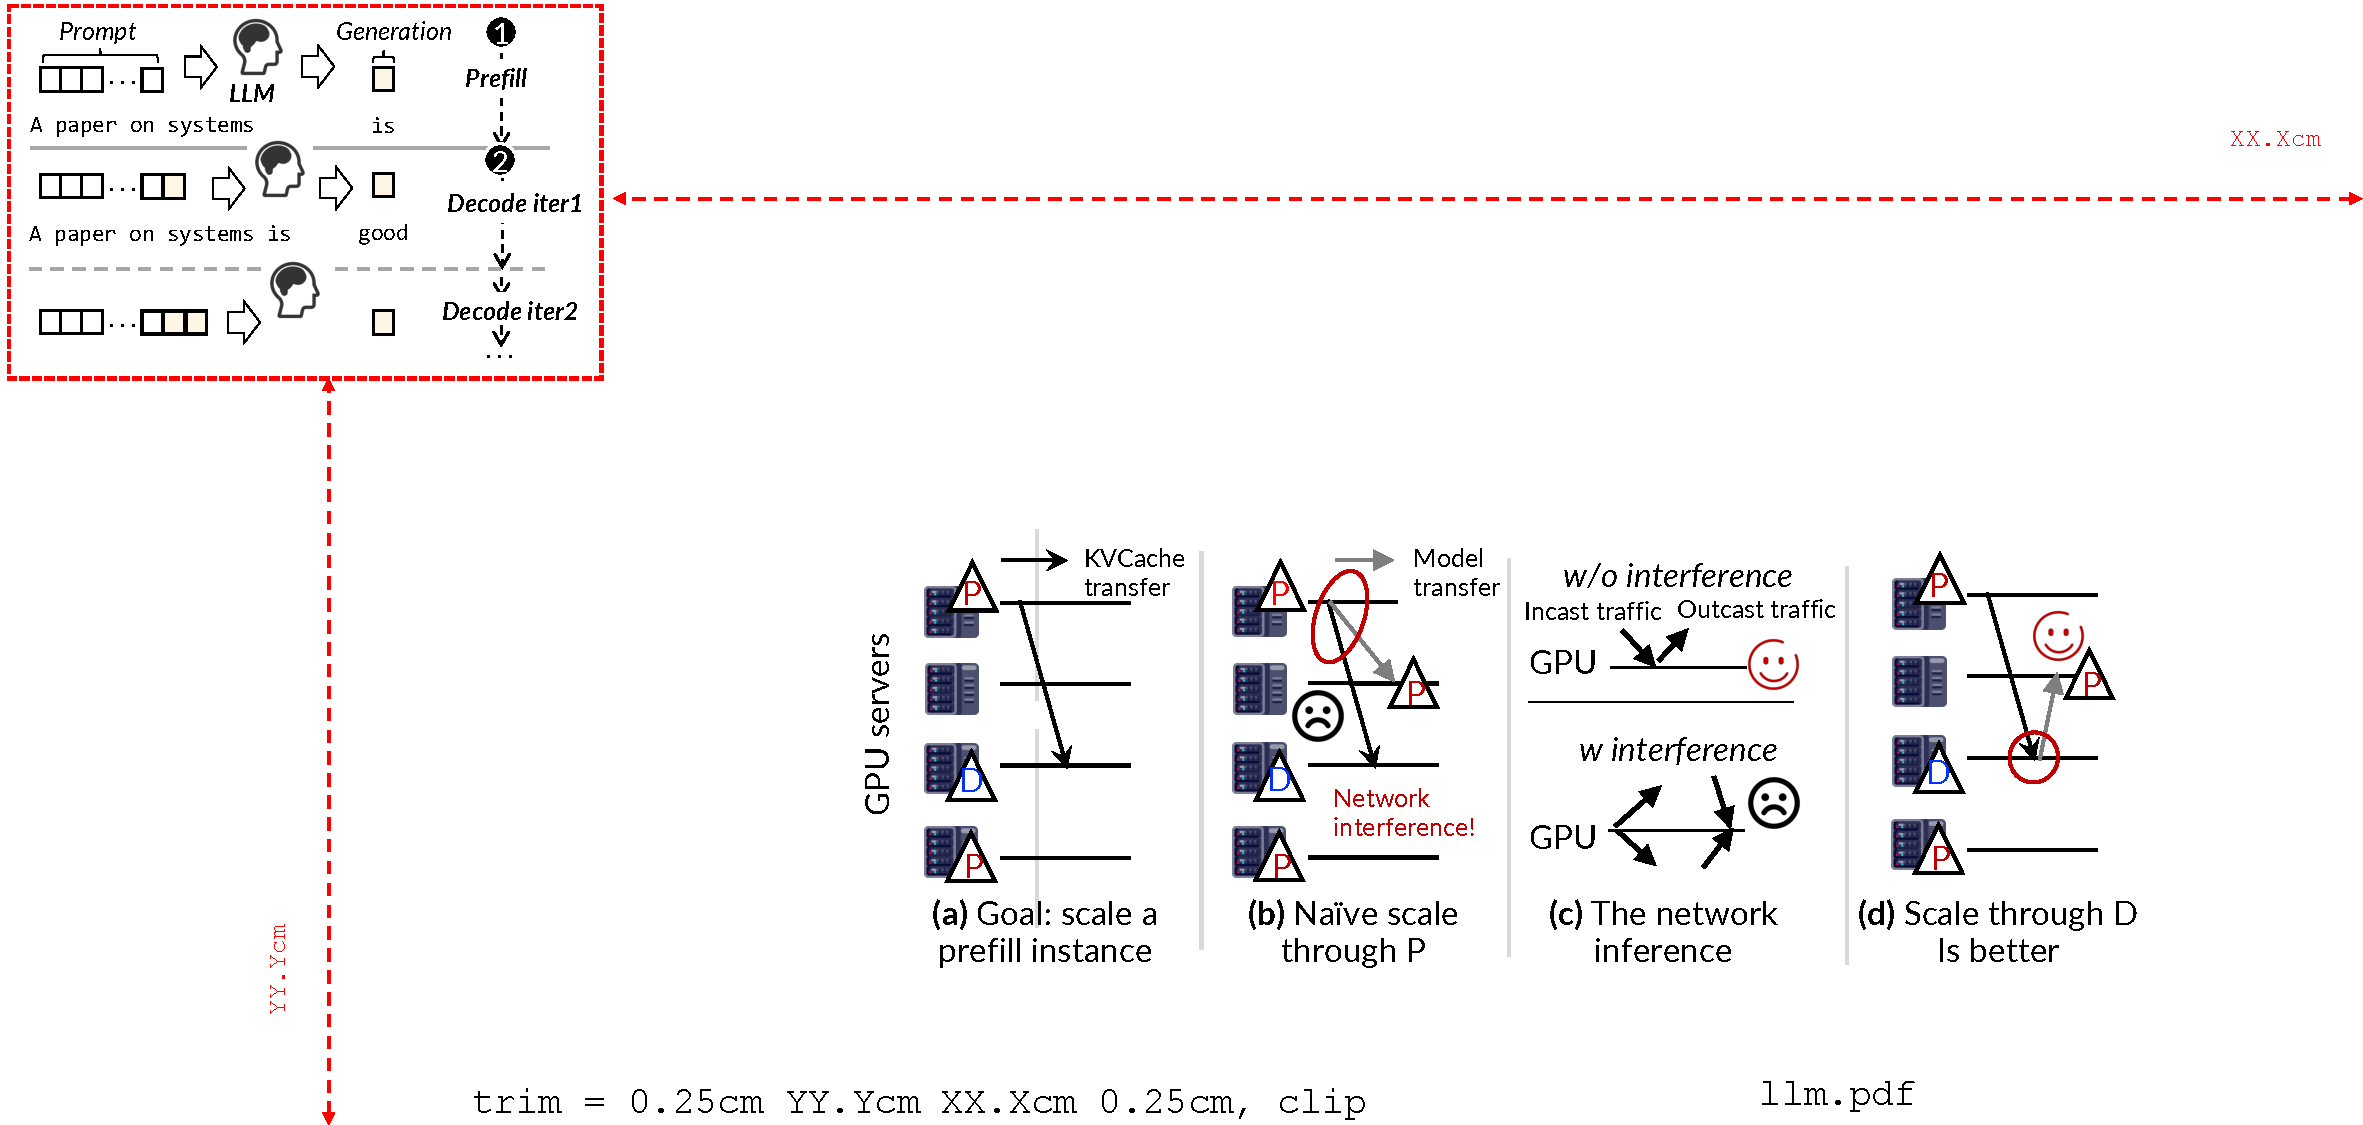
\includegraphics[width=.9\columnwidth,trim=0.25cm 12.7cm 30cm 0.25cm,clip]{figs/llm.pdf}
    \caption{LLM 处理请求过程示意图。}
    \label{fig:bg-llm}
\end{figure}

\nospacestitle{LLM 服务。}
如\fig{fig:bg-llm}所示，大语言模型（LLM）以自回归方式处理请求。给定一个请求（或一批请求），其中每个请求都包含多个 token（即提示词），模型首先执行预填充阶段，通过一次前向传播生成第一个 token（\ding{182}）。随后模型进入解码阶段（\ding{183}），通过多次前向传播迭代生成余下 token；当模型输出序列结束（EOS）token 时，迭代终止。在每次迭代中，输入既包含原始提示词，也包含此前生成的所有 token。

\begin{figure}[!t]
    \centering
    \includegraphics[width=\columnwidth,trim=0.25cm 11.1cm 26.4cm 0.25cm,clip]{figs/kvcache.pdf}
    \caption{示意图：\ding{182} 预填充请求（Req\#0）产生的 {\kvcache} 如何被 Req\#0 的解码阶段复用；\ding{183} {\kvcache} 如何被未来请求（Req\#1）的预填充阶段复用。}
    \label{fig:bg-kvcache}
\end{figure}

\stitle{KVCache（\kvcache）。}
如\fig{fig:bg-kvcache}所示，LLM 的一次前向传播包含三个步骤~\cite{DBLP:conf/nips/VaswaniSPUJGKP17}：（1）通过矩阵乘法计算 Q、K、V 矩阵；（2）利用 Q 与 K 得到注意力分数；（3）将注意力分数与 V 矩阵结合，产生注意力结果。这些步骤计算密集。由于具有相同 token 的输入共享相同 K、V 矩阵（见\ding{182}），所有 LLM 服务系统都会在 GPU 上缓存预填充阶段产生的 K、V 矩阵，以节省计算时间；随后同一请求在解码阶段复用这些缓存的 K、V 矩阵，避免重复计算，因而它们被称为 {\kvcache}。

\stitle{{\kvcache} 缓存与 {\kvcache} 块。}
除处理单个请求时在预填充和解码阶段之间复用 {\kvcache} 外，只要不同请求共享相同 token 前缀，{\kvcache} 也可跨请求复用。如\fig{fig:bg-kvcache}中的\ding{183}所示，“A paper on”的 K、V 值在 Req\#0 与 Req\#1 中完全相同。因此，即使 Req\#0 已完成解码，仍可保留其 {\kvcache} 供 Req\#1 使用，从而显著改善 Req\#1 的响应时间（也称首 token 时间，TTFT）：其预填充阶段只需计算“AI is”的 K、V。由于节省了计算，{\kvcache} 缓存还会提高服务吞吐量。基于这些原因，现有服务系统都会缓存已完成请求的 {\kvcache}。本文称这种方法为 {\kvcache} 缓存~\cite{vllm,cachedattention,promptcache,sglang,DBLP:journals/corr/abs-2404-12457,DBLP:conf/sigcomm/LiuLCRHZDY0AMHH24,DBLP:journals/corr/abs-2403-14401}，尽管它也常被称为前缀缓存或提示词缓存。{\kvcache} 可以缓存在 GPU 内存、主机内存（或远程机器内存），甚至 SSD 中~\cite{vllm,cachedattention,DBLP:journals/corr/abs-2403-14401}。

逐 token 检查前缀匹配可能代价很高，因此现有 {\kvcache} 系统以\emph{块}为缓存粒度，每个块包含可配置数量 token 的 KV。例如，vLLM~\cite{vllm} 默认将 16 个 token 组成一个块。

\stitle{多轮服务。}
通过多轮对话与 LLM 交互，是改善服务质量的一种常见模式~\cite{wu2024autogen,wang2023mint}。具体而言，收到 LLM 的生成结果后，用户可能使用新提示词发起下一轮请求。由于 LLM 需要此前的对话上下文，服务系统会将先前各轮请求的输入和输出拼接到新请求输入中，再将新输入送入 LLM。为帮助管理多轮请求历史，同一多轮对话中的请求通常归为一个\emph{会话}。由于当前 LLM 系统会有意把历史输入输出附加为每个新请求的前缀，多轮请求自然会复用先前轮次的 {\kvcache}。
